%%%%%%%%%%%%%%%%%%%%%%%%%%%%%%%%%%%%%%%%%%%%%%%%%%%%%%%%%%%%%%%%%%%%%%%%%%%%%%%%%%%%%%%%%%%%%%%%
%
% CS484 Written Question Template
%
% Acknowledgements:
% The original code is written by Prof. James Tompkin (james_tompkin@brown.edu).
% The second version is revised by Prof. Min H. Kim (minhkim@kaist.ac.kr).
%
% This is a LaTeX document. LaTeX is a markup language for producing
% documents. Your task is to fill out this document, then to compile
% it into a PDF document.
%
%
% TO COMPILE:
% > pdflatex thisfile.tex
%
% If you do not have LaTeX and need a LaTeX distribution:
% - Personal laptops (all common OS): www.latex-project.org/get/
% - We recommend latex compiler miktex (https://miktex.org/) for windows,
%   macTex (http://www.tug.org/mactex/) for macOS users.
%   And TeXstudio(http://www.texstudio.org/) for latex editor.
%   You should install both compiler and editor for editing latex.
%   The another option is Overleaf (https://www.overleaf.com/) which is
%   an online latex editor.
%
% If you need help with LaTeX, please come to office hours.
% Or, there is plenty of help online:
% https://en.wikibooks.org/wiki/LaTeX
%
% Good luck!
% Min and the CS484 staff
%
%%%%%%%%%%%%%%%%%%%%%%%%%%%%%%%%%%%%%%%%%%%%%%%%%%%%%%%%%%%%%%%%%%%%%%%%%%%%%%%%%%%%%%%%%%%%%%%%
%
% How to include two graphics on the same line:
%
% \includegraphics[\width=0.49\linewidth]{yourgraphic1.png}
% \includegraphics[\width=0.49\linewidth]{yourgraphic2.png}
%
% How to include equations:
%
% \begin{equation}
% y = mx+c
% \end{equation}
%
%%%%%%%%%%%%%%%%%%%%%%%%%%%%%%%%%%%%%%%%%%%%%%%%%%%%%%%%%%%%%%%%%%%%%%%%%%%%%%%%%%%%%%%%%%%%%%%%

\documentclass[11pt]{article}

\usepackage[english]{babel}
\usepackage[utf8]{inputenc}
\usepackage[colorlinks = true,
            linkcolor = blue,
            urlcolor  = blue]{hyperref}
\usepackage[a4paper,margin=1.5in]{geometry}
\usepackage{stackengine,graphicx}
\usepackage{fancyhdr}
\setlength{\headheight}{15pt}
\usepackage{microtype}
\usepackage{times}
\usepackage{booktabs}

% From https://ctan.org/pkg/matlab-prettifier
\usepackage[numbered,framed]{matlab-prettifier}

\frenchspacing
\setlength{\parindent}{0cm} % Default is 15pt.
\setlength{\parskip}{0.3cm plus1mm minus1mm}

\pagestyle{fancy}
\fancyhf{}
\lhead{Homework Writeup}
\rhead{CS484}
\rfoot{\thepage}

\date{}

\title{\vspace{-1cm}Homework 3 Writeup}


\begin{document}
\maketitle
\vspace{-3cm}
\thispagestyle{fancy}

\section*{Instructions}
\begin{itemize}
  \item Describe any interesting decisions you made to write your algorithm.
  \item Show and discuss the results of your algorithm.
  \item Feel free to include code snippets, images, and equations.
  \item Use as many pages as you need, but err on the short side If you feel you only need to write a short amount to meet the brief, th
  \item \textbf{Please make this document anonymous.}
\end{itemize}

\section*{Bayer to RGB Demosaicing}
The first part of this assignment was to implement Bayer to RGB Demosaicing, which involves decoding the color information stored in a flat image and constructuring the colored image. I have used the simple bilinear interpolation method to construct the colored image. The algorithm is simple: for a pixel that does have a color value for a particular color, take that as the value for that color. Otherwise, take the average of the values of its neighbouring pixels for that color. The results were as follows:

\begin{figure}[h]
    \centering
    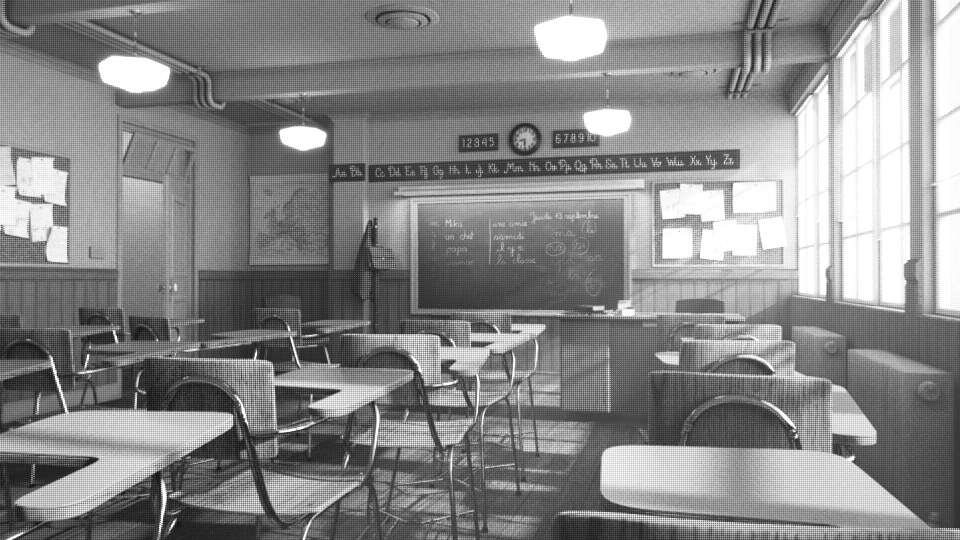
\includegraphics[width=5cm]{bayer_before.png}
    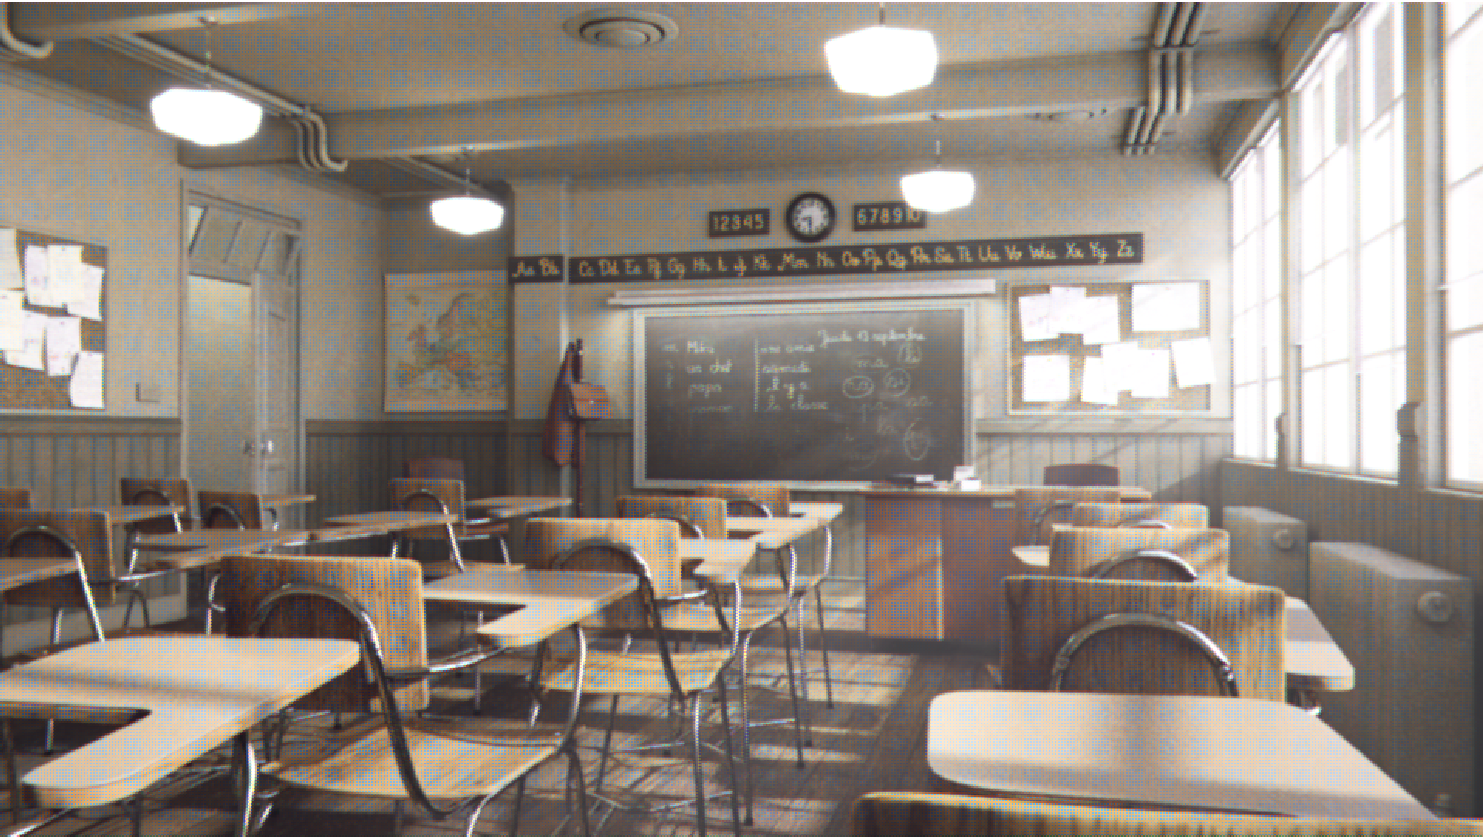
\includegraphics[width=5cm]{bayer_after.png}
    \caption{\emph{Left:} Before Demosaicing \emph{Right:} After Demosaicing}
    \label{fig:result1}
\end{figure}

A particular difficulty that I've faced was with the \emph{uint8} data type. Here is a snippet of the initial code that I wrote:
\begin{lstlisting}[style=Matlab-editor]
B = (mat(x - 1, y - 1) + mat(x + 1, y - 1) + mat(x - 1, y + 1) + mat(x + 1, y + 1)) / 4;
\end{lstlisting}

This code turned out to produce problematic results because the matrix elements were of type 'uint8'. If the sum of these 4 numbers are over 255, B would eventuall contain just 255 / 4, which is not accurate. The solution was to divide each values by 4, as this code snippet shows:
\begin{lstlisting}[style=Matlab-editor]
B = mat(x - 1, y - 1) / 4 + mat(x + 1, y - 1) / 4 + mat(x - 1, y + 1) / 4 + mat(x + 1, y + 1) / 4;
\end{lstlisting}

\section*{Calculating Fundamental Matrix with Normalized 8 Point Algorithm}
The second task was to estimate the fundamental matrix between two stereo images with the \emph{Normalized 8 Point Algorithm}. Assuming that we take two matrices \emph{pts1, pts2} containing 2D points, the process for this algorithm is as follows:
\begin{enumerate}
    \item Convert \emph{pts1} and \emph{pts2} homogenous coordinates.
    \item Normalize \emph{pts1} and \emph{pts2}.
    \item Extract eigenvector F corresponding to least singular value, and rearrange it to be 3x3.
    \item Perform SVD on F = USV', and enforce rank 2 on S by setting S(3,3) = 0.
    \item Retrieve fundamental matrix F in original coordinate and normalize F.
\end{enumerate}
Now we use this fundamental matrix for rectifying stereo images.
\section*{Rectifying Stereo Images}
Using 2 homography matrices for each of the images, we now rectify the two images. We use \texttt{projective2d} to retrieve the projective matrix from the two homography matrices. Using these projective matrices, we then translate the corners of 2 images to find out the translated corners for each image. This is for making sure that the two images have the same size. Using the 8 translated corners, we calculate the width and height of the two images. Finally, we translate the two images with the width and height information using \texttt{imwarp} and \texttt{imref2d}.

The following is the result of rectification.
\begin{figure}[h]
    \centering
    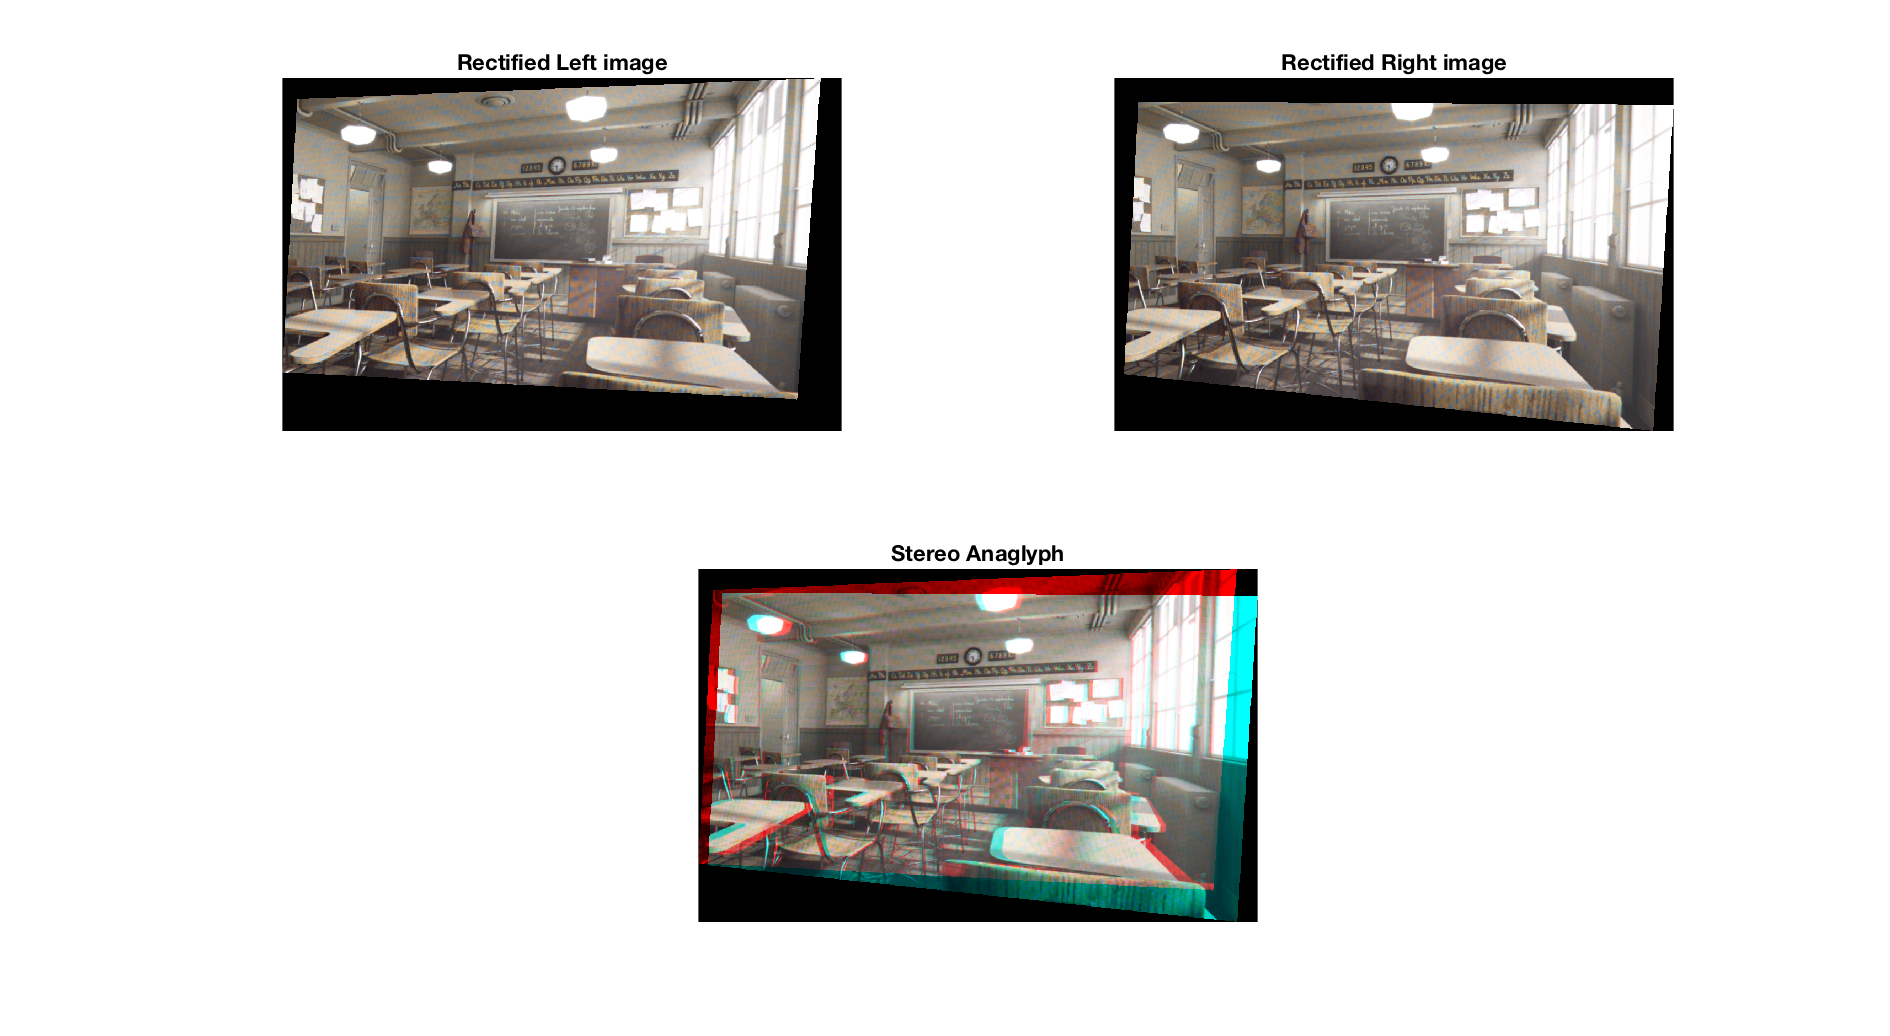
\includegraphics[width=8cm]{rectified.png}
    \caption{Result of stereo rectification}
    \label{fig:result1}
\end{figure}

\section*{Calculating Disparity Map}
The disparity map was calculated by using NCC as matching cost. For every pixel in the left image, it searches through the pixels that are on its horizontal line. Since a higher NCC means low disparity, we find the pixel in the right window that has the largest NCC value and take the difference in width as disparity. The following is the result of disparity map.

\begin{figure}[h]
    \centering
    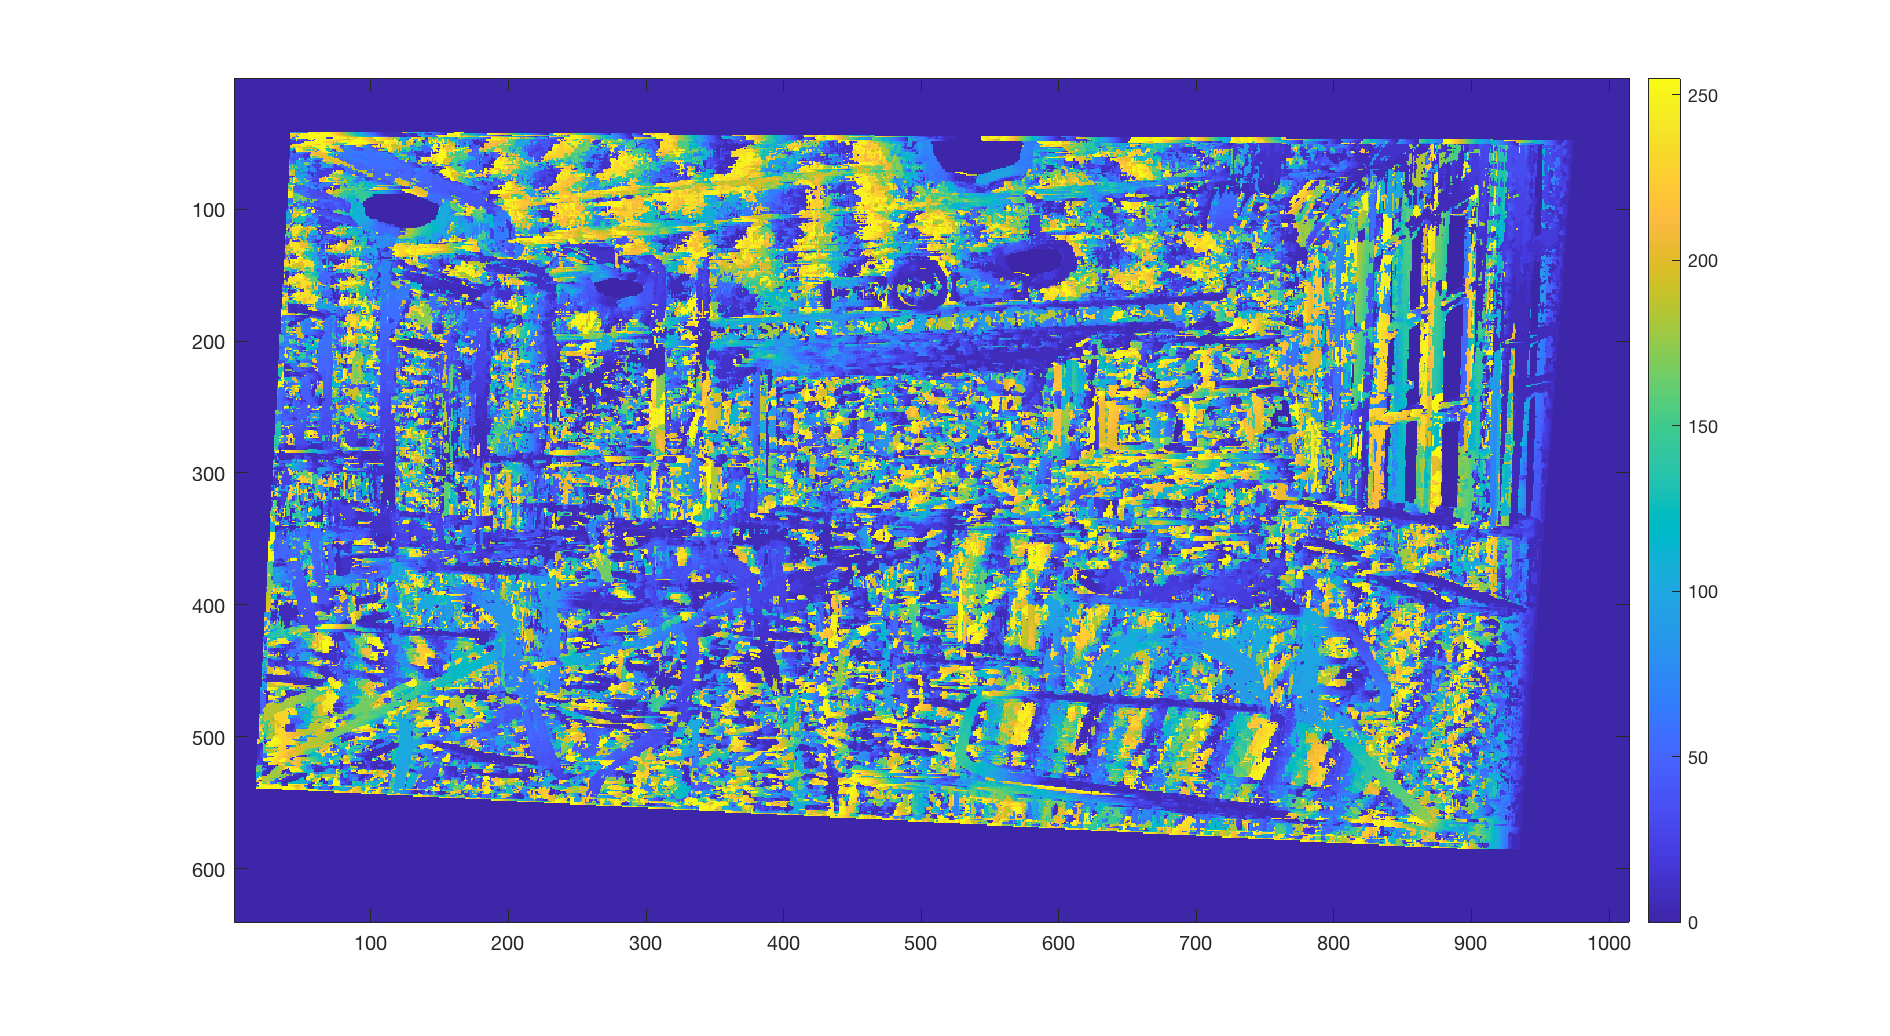
\includegraphics[width=8cm]{disparity.png}
    \caption{Disparity Map}
    \label{fig:result1}
\end{figure}

\end{document}
